% --------------------------------------------------------------
%                         Template HW
% --------------------------------------------------------------
\documentclass[a4paper, 12pt]{article} %draft = show box warnings
\usepackage[utf8]{inputenc} % Accept different input encodings [utf8]
\usepackage[T1]{fontenc}    % Standard package for selecting font encodings
%\usepackage[a4paper, total={6.5in,10.2in}]{geometry} % Flexible and complete interface to document dimensions
\renewcommand{\baselinestretch}{1.3} 

% --------------------------------------------------------------
%                       Packages
% --------------------------------------------------------------
\usepackage{graphicx} % Import images
\usepackage[linktoc=all]{hyperref} % Create hyperlinks
\usepackage{float} % Good placement for float objects
\usepackage[export]{adjustbox} % Positioning figures
%\usepackage{amsmath,amsthm,amssymb} % American Mathematics Society facilities
\usepackage[fancysections,titlepage,sectionmark]{polytechnique}

% --------------------------------------------------------------
%                         Languages
%			Change also the exercise environment
% --------------------------------------------------------------
%\usepackage[english]{babel} % Multilingual support [english]
\usepackage[french]{babel} % Multilingual support [french]
%\usepackage[brazilian]{babel} % Multilingual support [pt-BR]

% --------------------------------------------------------------
%                         Fonts
% --------------------------------------------------------------
%\usepackage{lmodern} % Good looking T1 font
%\usepackage{mathpazo} % Hermann Zapf's Palatino font
%\usepackage{kpfonts} % Kepler font
%\usepackage{mathptmx} % Times New Roman Like Font
%\usepackage{eulervm} %  AMS Euler (eulervm) math font.

% --------------------------------------------------------------
%                       Begin Document
% --------------------------------------------------------------

\begin{document}

\title{Rapport de stage en entreprise}
\subtitle{Thales Research \& Technology}
\author{
\begin{tabular}{ccc}
	\textbf{Stagiaire}
	\\
	Alexandre RIBEIRO JOÃO MACEDO
	\\	
	\textbf{Tuteur en entreprise} 
	\\
	M. Jean-Marc MOTA
	\\
	\textbf{Référent FX}
	\\
	M. Olivier DELASSUS
\end{tabular}
}
\date{19 septembre 2017}
\maketitle

\addcontentsline{toc}{section}{Executive Summary}
\section*{Executive Summary}
Le stage de découverte d'entreprise fait comme une composant obligatoire du curriculum de deuxième année du cycle d'ingénieur polytechnicien est essentielle à formation du futur ingénieur. Dans le cadre de ce stage, l'élève a l'opportunité de développer un travail pour une entreprise et de découvrir le monde du travail. Ce qui est bien différente de celui de l'école.

Mon stage a été fait à Thales Recherche et Technologie dans le Laboratoire de Systèmes Embarqué Critique, où j'ai pu faire un projet dans le domaine de méthodes formelles. Plus spécifiquement, j'ai travaillé avec l'écriture des spécifications formelles des algorithmes distribués, leur \textit{Model Checking} ("Vérification de modèle") et l'implémentation d'une visualisation pour les résultats de ce dernier. Le \textit{Model Checking} est important pour trouver les erreurs logiques dans les algorithmes qui sont difficile à prévoir pendant sa conception et qui peuvent être dangereuses s'ils sont utilisent dans la production.

Pendant mon stage de douze semaines, de 12 juillet 2017 à 31 août 2017, j'ai été orientée par M. Jean-Marc Mota qui a beaucoup m'aidé dans le côté technique, mais qui a aussi me donné des conseilles pour la vie professionnelle. Un autre expérience intéressant pendant le stage a été le Forum des Stagiaires de Thales, où les stagiaires ont été donnés des conseilles pour la réussit professionnelle.

Le but de ce rapport est de décrire les expérience vécues pendants ces douze semaines et le apport de ces expériences dans ma formation.

\newpage
\addcontentsline{toc}{section}{Remerciements}
\section*{Remerciements}
Je voudrais remercie M. Jean-Marc Mota mon tuteur responsable par mon stage

\newpage
\tableofcontents

\newpage
\section{Introduction}
La révolution du numérique est un phénomène qui a eu leur place pendant les trente dernières années et, à chaque jour, les systèmes informatiques ont plus d'influence et responsabilité sur la vie des personnes. Alors, il n'est pas étonnant que un grand nombre de gens aient un intérêt par ce domaine. Dans mon cas, j'ai choisi le laboratoire de systèmes embarqués critiques de Thales Research \& Technology (TRT) parce que cela a été l'opportunité de voir comment les applications critiques sont développés dans l'industrie.

Cela a été un bon complément à les études en informatique que j'ai réalisé à l'école et aussi cela a été l'opportunité d'être en contact avec le monde organisationnel des grandes sociétés comme Thales. Cette expérience a aussi m'aidé à clarifier quelques doutes sur mon parcours et de commencer le troisième année avec un projet professionnelle bien définit. 

Pour résumer, le stage m'apporté beaucoup de connaissance technique, mais aussi de développement personnelle - professionnelle.

\newpage
\section{Présentation de Thales}
 Thales Group est une société anonyme et un des leaders mondiaux des équipements destinés à des industries de l'aéronautique, de l'espace, de la défense, de la sécurité et des modes de transport. Elle est présente dans 56 pays et emploie plus de 64000 salariés.
 Le groupe 
 
\subsection{Thales Reseach \& Technology}
Thales 

\subsection{L'égalité hommes - femmes}
D'après \cite{thales}, Thales a mis en ouvre une politique de l'égalité homme - femme. Notamment, depuis 31 décembre 2016 le Conseil Thales est composé par 8 femme, ce que représente 50\% des 16 administrateurs dans le Conseils. Par contre, seulement 30\% des salariés de Thales dans le monde sont des femmes.

Dans mon avis personnel basé uniquement sur l'observation du environnement de travail, la proportion homme - femme change avec le secteur de l'entreprise. Par exemple, dans le secteur de RH il y une grande proportion de femmes. Par contre, dans le secteur de ingénierie est claire que la quantité d'hommes est plus grand que celui de femmes. Entre les physicien, cette proportion est plus équilibre. 

C'est intéressent la position de Thales au sens des ces politiques d'intégration de femmes. Celas a déjà donnés des résultats importantes non seulement pour le nombre de salaries de chaque genre, mais aussi pour la égalité entre les salaires. Une analyse très complète de ces politiques et ses résultats est disponible en \cite{thales}

\subsection{Forum Stagiaire de Thales}
Le Forum Stagiaire est un événement que s'est déroulé le juin 2017 à Thales Université à Jouy-en-Josas, où les stagiaires de Thales ont été invités à des conférences dont l'objectif étaient donner les conseilles sur CV, le profile LinkedIn, les entretiens d'embauche. Il y avait aussi des ateliers photos, les ateliers de CV et les simulations d'entretien.

Cela a été une opportunité unique de voir le point de vu des professionnelles de ressources humaines dans les procès d'embouche. Personnellement, après le forum j'ai gardé et déjà utilisé les conseilles donnés pendant le Forum et je suis sure que cela m'aidera dans le futur. Malheureusement, le Forum Stagiaire 2017 fut le dernier Forum Stagiaire à Thales Université.

\begin{figure}[H]
	\centering
	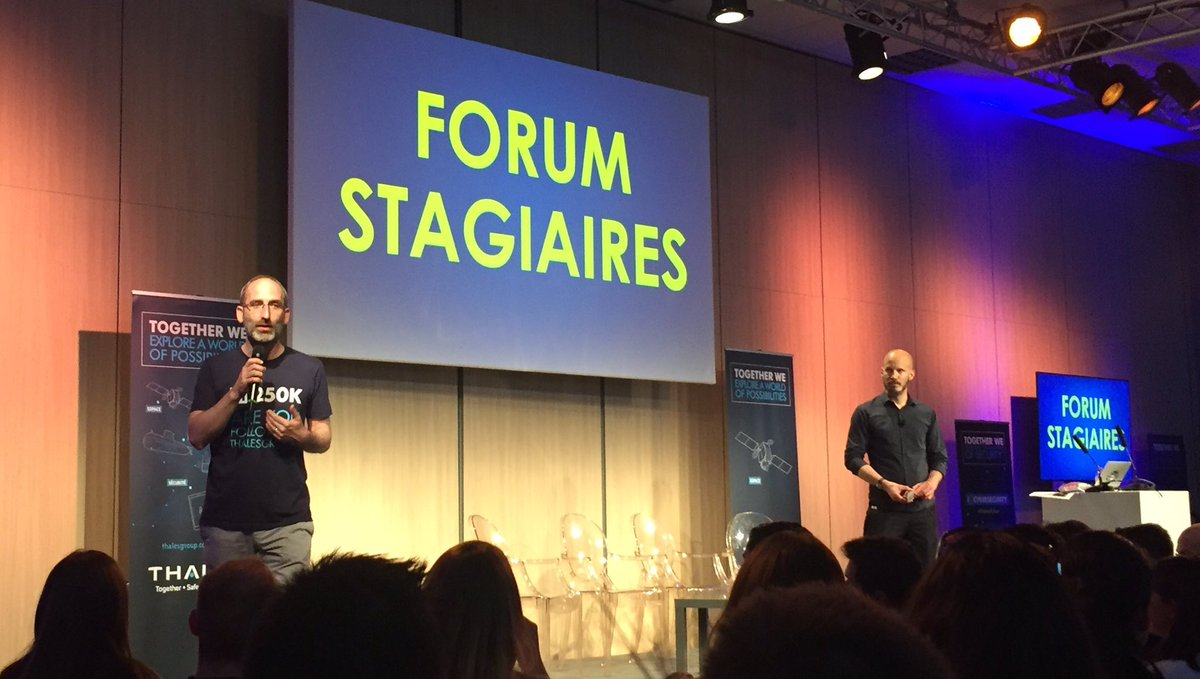
\includegraphics[width=\textwidth]{images/forum_stagiare.jpg}
	\caption{Le Forum Stagiaire à Thales Université}
	\label{forum_stagiare}
\end{figure}

\newpage
\section{Mission du stage}
\subsection{Le algorithme de consensus Raft}
\subsection{La langage TLA+ et le \textit{Model checker} TLC}
\subsection{Le algorithme de consensus Bully}

\newpage
\section{Enseignement}

\subsection{Apport Personnelle}

\subsection{Apport Professionnelle}


\newpage
\section{Conclusions}

\newpage

\begin{thebibliography}{3}
\addcontentsline{toc}{section}{Références}	
	\bibitem{thales} %% To cite use \cite{example}
	Thales Group,  
	\textit{Document de référence 2016}.
	\url{https://www.thalesgroup.com/sites/default/files/asset/document/thales_ddr_2016_vf.pdf}
	
	\bibitem{raft} 
	Raft Consensus Algorithm webpage,
	\url{https://raft.github.io/}
	
	\bibitem{bully} 
	Bully Consensus Algorithm wikipedia,
	\url{https://en.wikipedia.org/wiki/Bully_algorithm}
\end{thebibliography}
\end{document}
